\chapter{Introduction}
\label{chpt:intro}

Due to its high accuracy, \acrfull{dnn} is widely adopted in image classification cloud services, object detection applications, \acrfull{llm}, etc. Meanwhile, as computational resources grow on edge devices, intelligent robots benefit from deep learning models to obtain a more comprehensive perception of the environment than traditional robots. However, deep learning models are vulnerable to adversarial attacks that can manipulate model outputs by adding carefully crafted small perturbations to model inputs.

This chapter first introduces how deep learning models are employed in autonomous driving systems and clinical diagnosis applications. Then, we review existing adversarial attacks, including white-box attacks and black-box attacks. Lastly, we discuss unexplored research questions and summarize the structure of the thesis.

% For instance, the Amazon Kiva Robot and Alibaba Quicktron Robot can help warehouse staffs find desired items by moving goods shelves. Each robot can perceive the surrounding environment to avoid collisions with other robots, and receive commands from warehouse staff via cloud servers. On the other hand, autonomous driving research teams from Waymo (formerly the Google self-driving car project), Tesla, etc intend to achieve autonomous navigation without human interference.

% On the other hand, the development of physics engines and realistic renderers makes it feasible to simulate complex robots in simulators. Reinforcement learning that learns from trial and error, can now be trained and verified in a virtual environment before deploying to the physical world.


\section{Deep Learning}
\label{sec:deep_learning}

% \begin{figure}[H]
% \centering
% \begin{subfigure}[b]{0.485\textwidth}
%     \centering
%     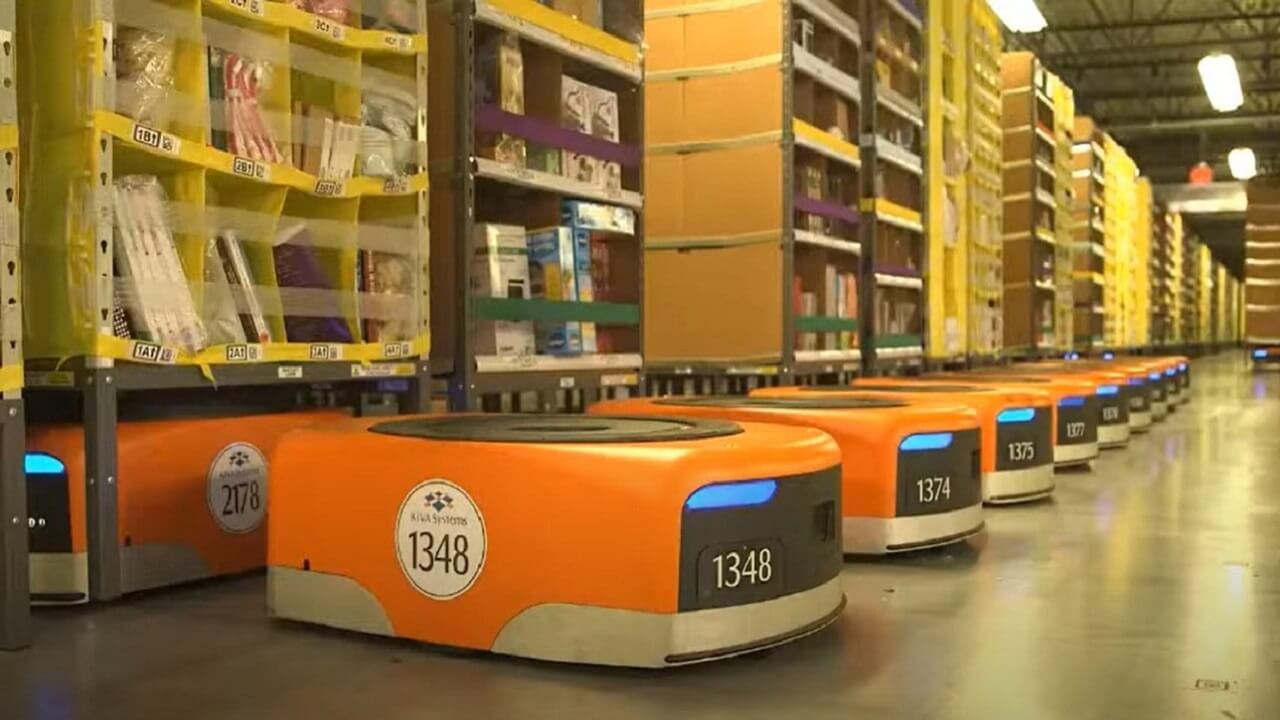
\includegraphics[width=\textwidth]{figures/chapter_intro/amazon_kiva.jpg}
%     \caption{Amazon Kiva Robot}
%     \label{fig:kiva}
% \end{subfigure}
% \hfill
% \begin{subfigure}[b]{0.485\textwidth}
%     \centering
%     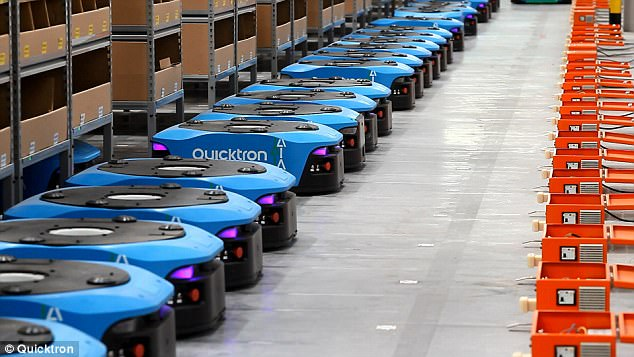
\includegraphics[width=\textwidth]{figures/chapter_intro/alibaba_quicktron.jpg}
%     \caption{Alibaba Quicktron Robot}
%     \label{fig:quicktron}
% \end{subfigure}
% \hfill
% \caption{Robots in warehouse.}
% \label{fig.robot}
% \end{figure}

% \begin{figure}[H]
% \centering
% \begin{subfigure}[b]{0.485\textwidth}
%     \centering
%     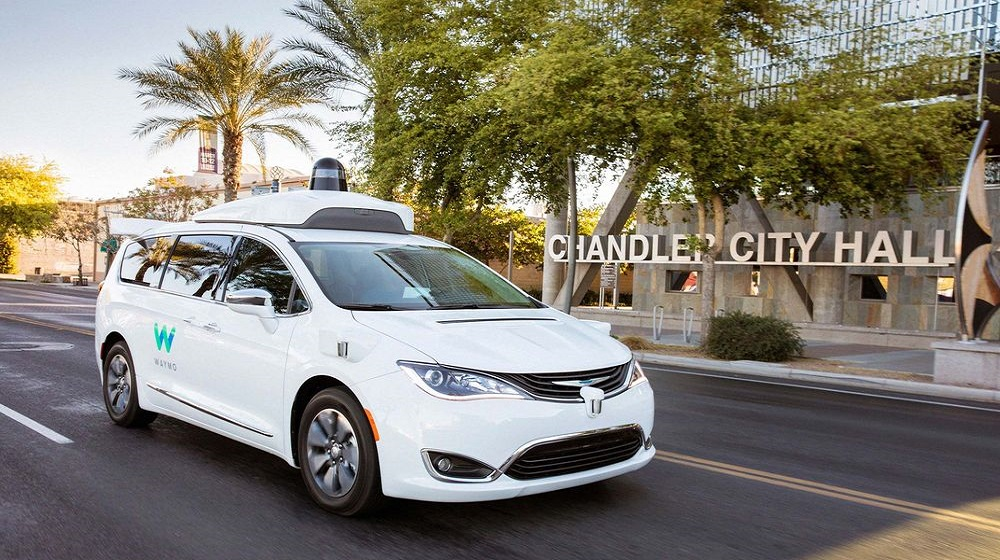
\includegraphics[width=\textwidth]{figures/chapter_intro/waymo.jpg}
%     \caption{Waymo (formerly Google self-driving project)}
%     \label{fig:waymo}
% \end{subfigure}
% \hfill
% \begin{subfigure}[b]{0.485\textwidth}
%     \centering
%     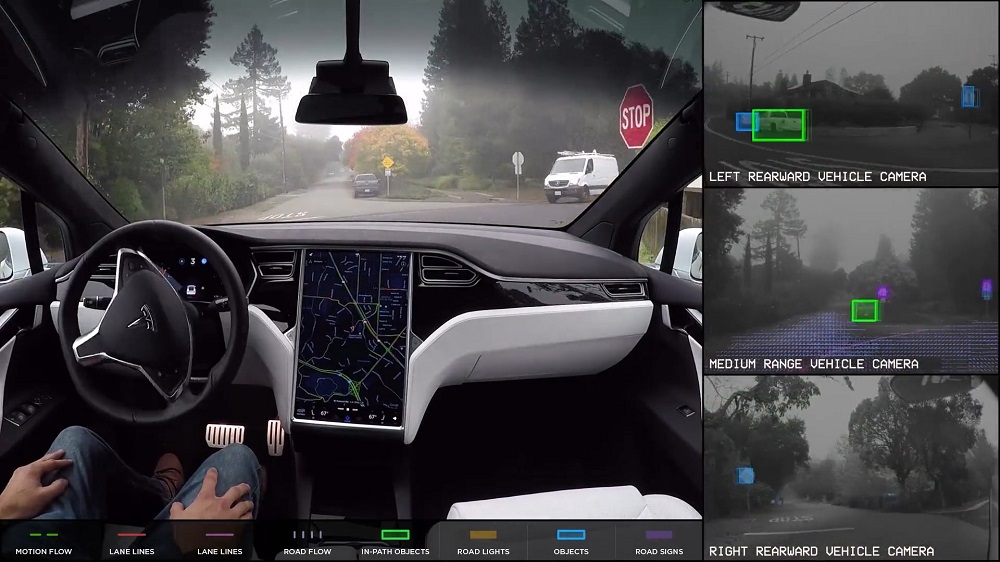
\includegraphics[width=\textwidth]{figures/chapter_intro/tesla_autopilot.jpg}
%     \caption{Tesla Autopilot}
%     \label{fig:tesla}
% \end{subfigure}
% \hfill
% \caption{Autonomous Driving Research}
% \label{fig.autonomous}
% \end{figure}

% As the research in deep neural networks advances, deep convolutional networks become feasible for automated driving tasks. Our research investigates the effect of adversarial attacks against deep learning models.

Autonomous Driving is an example of successful deep-learning applications. Following the established divide-and-conquer engineering principle, autonomous driving systems are commonly designed as modular systems that divide the driving task into sub-tasks: localization, perception, prediction, planning, and control. 

Through the localization module, the vehicle determines its position in the environment. The perception module enables vehicles to collect information and extract relevant knowledge from the environment. Then, the prediction module predicts future measurement, behavior, trajectory, etc. Lastly, the planning module makes purposeful decisions to achieve the goal, and the control module executes the planned actions \citep{pendleton2017perception}. Besides modular systems, end-to-end driving that maps inputs directly to steering commands has started to rise as an alternative to modular systems.

It is risky to attack real-world autonomous driving systems. The development of physics engines and realistic renderers makes it feasible to test adversarial attacks in photo-realistic simulators.
 
% \subsubsection{Deep Learning}
% \label{sec:deep_robot}

The CARLA simulator is an open-source platform for autonomous driving simulation based on the Unreal Game Engine (see Fig. \ref{fig:carla_intro}). It simulates various sensors such as depth camera, 3D lidar, and radar. Besides, the Carla simulator provides flexible Python API to interact with the virtual environments and supports \acrfull{ros} integration \citep{Dosovitskiy17}.

\begin{figure}[H]
\centering
\begin{subfigure}[b]{0.48\textwidth}
    \centering
    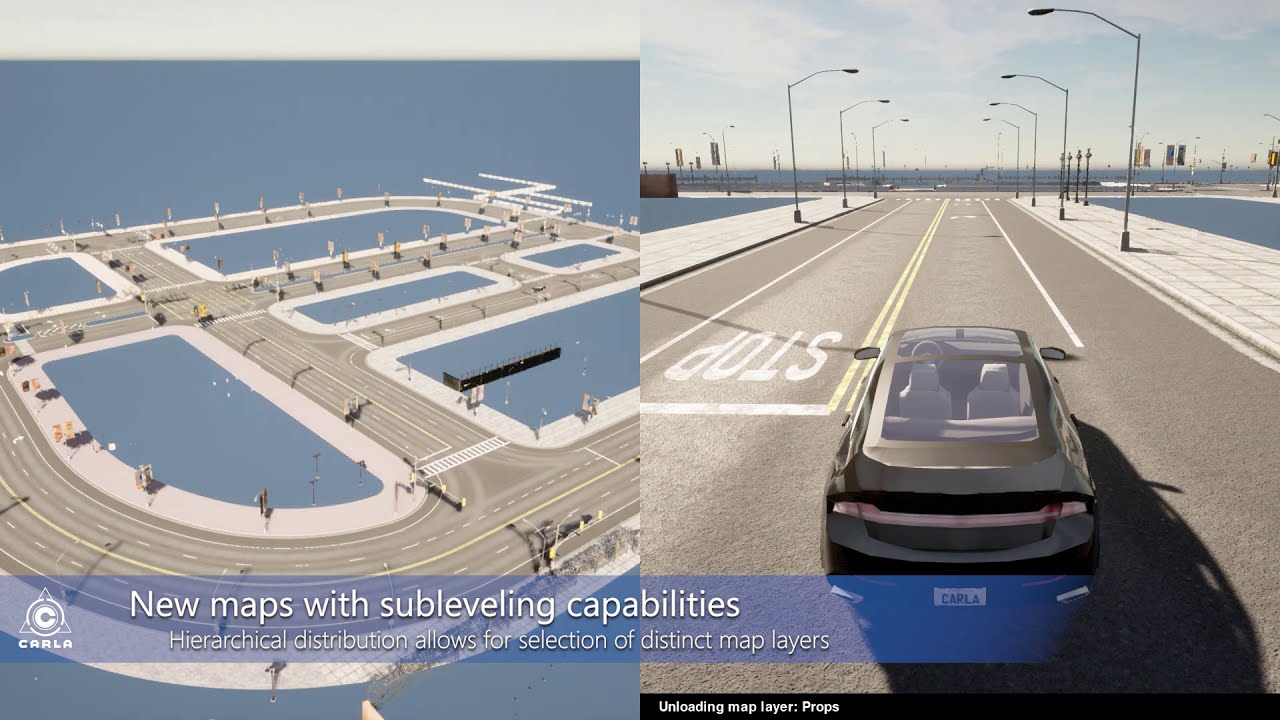
\includegraphics[width=\textwidth]{figures/chapter_intro/carla.jpg}
    \caption{CARLA Simulator \citep{Dosovitskiy17}}
    \label{fig:carla_intro}
\end{subfigure}
\hfill
\begin{subfigure}[b]{0.48\textwidth}
    \centering
    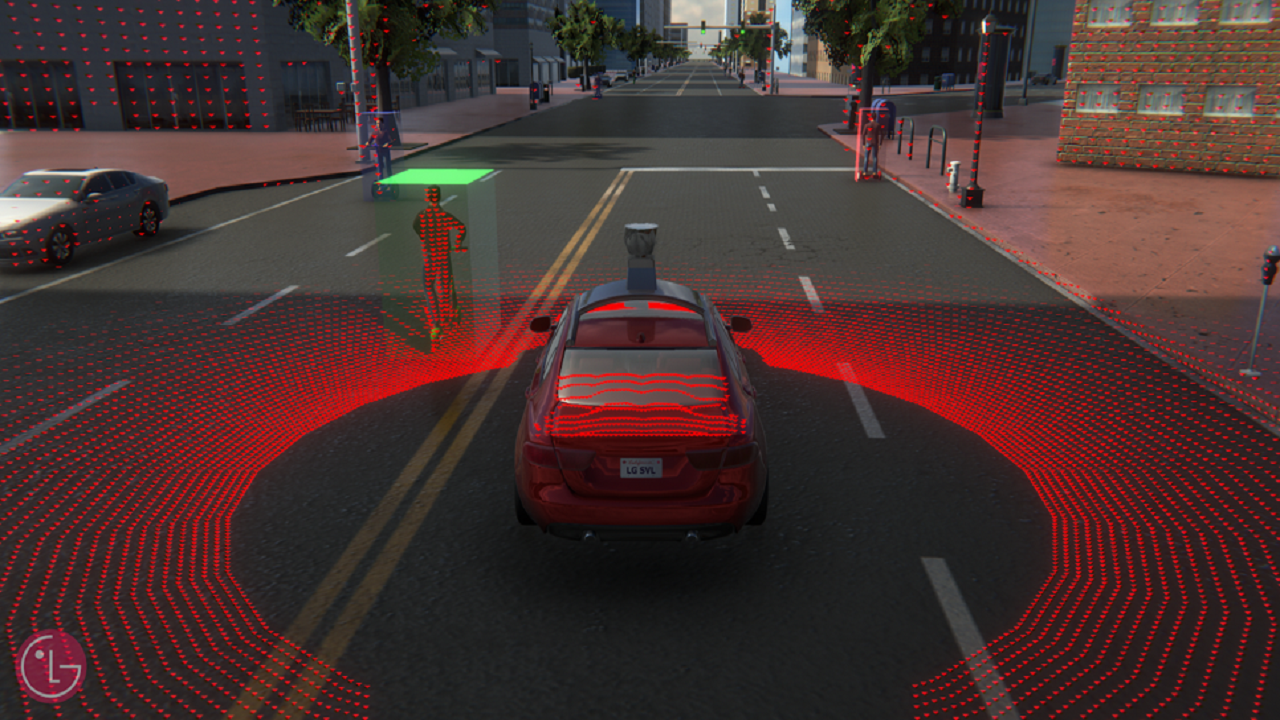
\includegraphics[width=\textwidth]{figures/chapter_intro/lgsvl.png}
    \caption{LGSVL Simulator\citep{rong2020lgsvl}}
    \label{fig:lvsvl}
\end{subfigure}
\hfill
\caption{Autonomous Driving Simulators}
\label{fig.simulator}
\end{figure}

The LGSVL is another autonomous vehicle simulation platform based on the Unity3D Game Engine (see Fig.\ref{fig:lvsvl}). It provides integration with the Baidu Apollo Platform \citep{rong2020lgsvl}. Both the CARLA simulator and LGSVL simulator focus on autonomous driving simulation. On the other hand, the Microsoft Airsim simulator provides virtual environments for both autonomous driving and drone simulation \citep{airsim2017fsr} (see Fig. \ref{fig.airsim}).

\begin{figure}[H]
\centering
\begin{subfigure}[b]{0.48\textwidth}
    \centering
    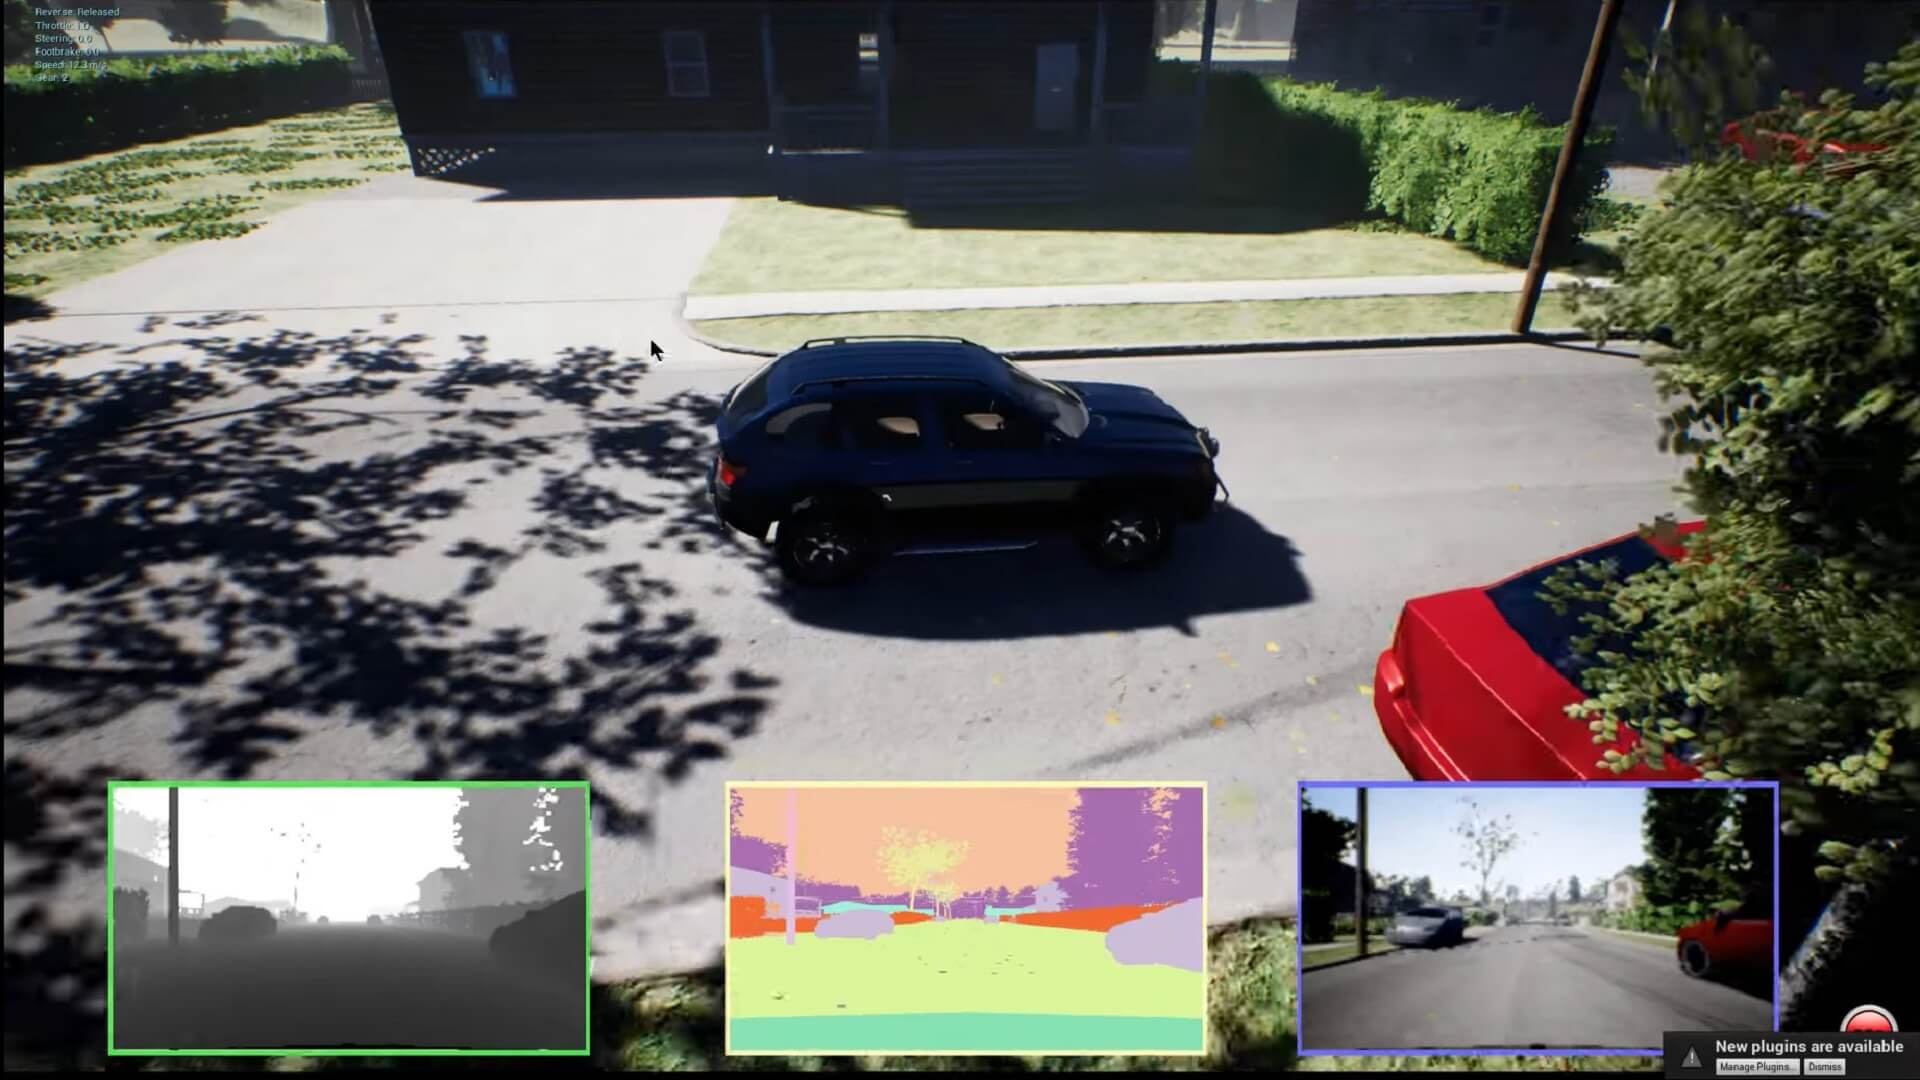
\includegraphics[width=\textwidth]{figures/chapter_intro/airsim_car.jpg}
    \caption{Airsim for Autonomous Vehicles}
    \label{fig:airsim_car}
\end{subfigure}
\hfill
\begin{subfigure}[b]{0.48\textwidth}
    \centering
    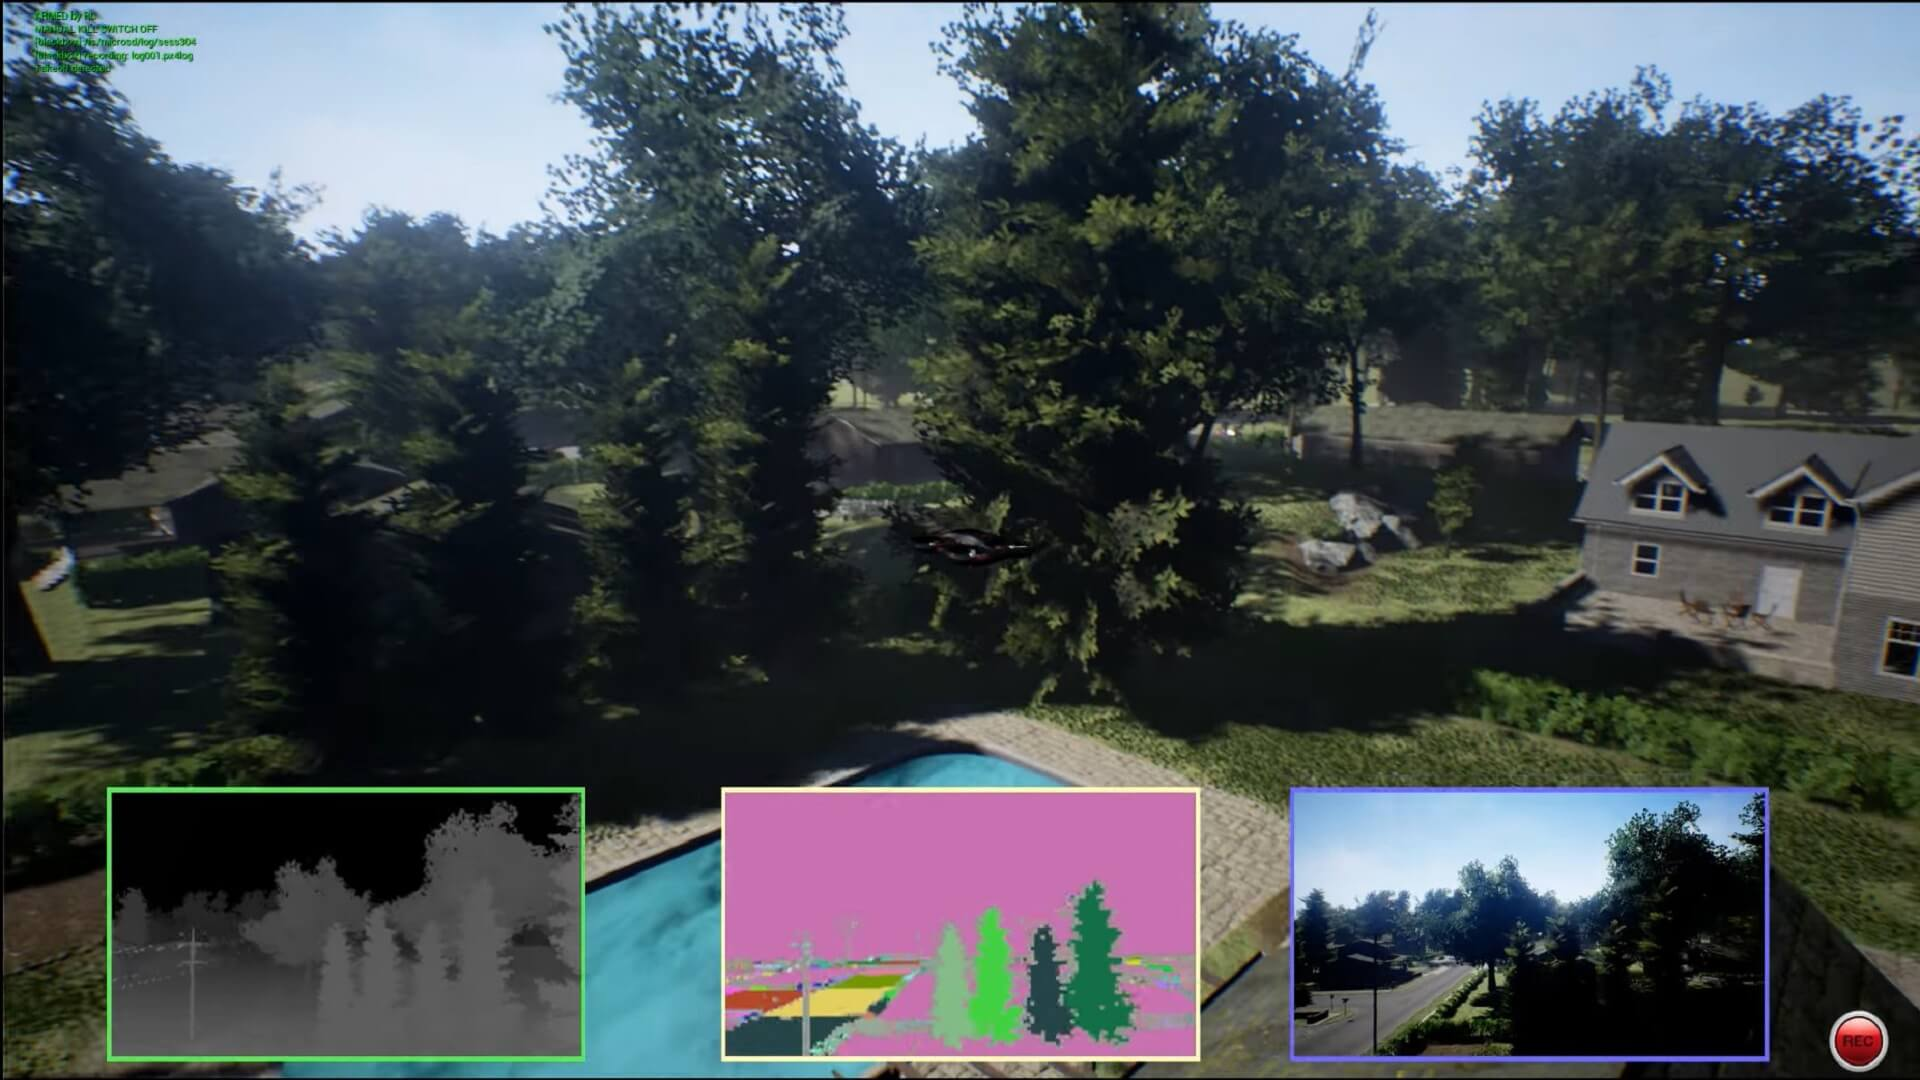
\includegraphics[width=\textwidth]{figures/chapter_intro/airsim_drone.jpg}
    \caption{Airsim for Drones}
    \label{fig:airsim_drone}
\end{subfigure}
\hfill
\caption{Microsoft Airsim Simulator \citep{airsim2017fsr}}
\label{fig.airsim}
\end{figure}

Besides autonomous driving, deep learning models are also widely used in medical applications, especially during the COVID-19 pandemic. With the rapid transmission of COVID-19, the demand for medical supplies goes beyond hospitals' capacity in many countries. Various diagnostic and predictive models are employed to release the pressure on healthcare workers.

% \clearpage

% \subsection{Reinforcement Learning}
% \label{sec:reinf_robot}

% Deep reinforcement learning can be integrated into robotic systems as well. Given observations of the environment under certain states, the agent (robot) takes actions to achieve objectives. Most reinforcement learning tasks are evaluated in games such as the Atari. Recently, the NVIDIA Issac Gym simulator makes large-scale reinforcement learning possible.

% \begin{figure}[H]
% \centering
% 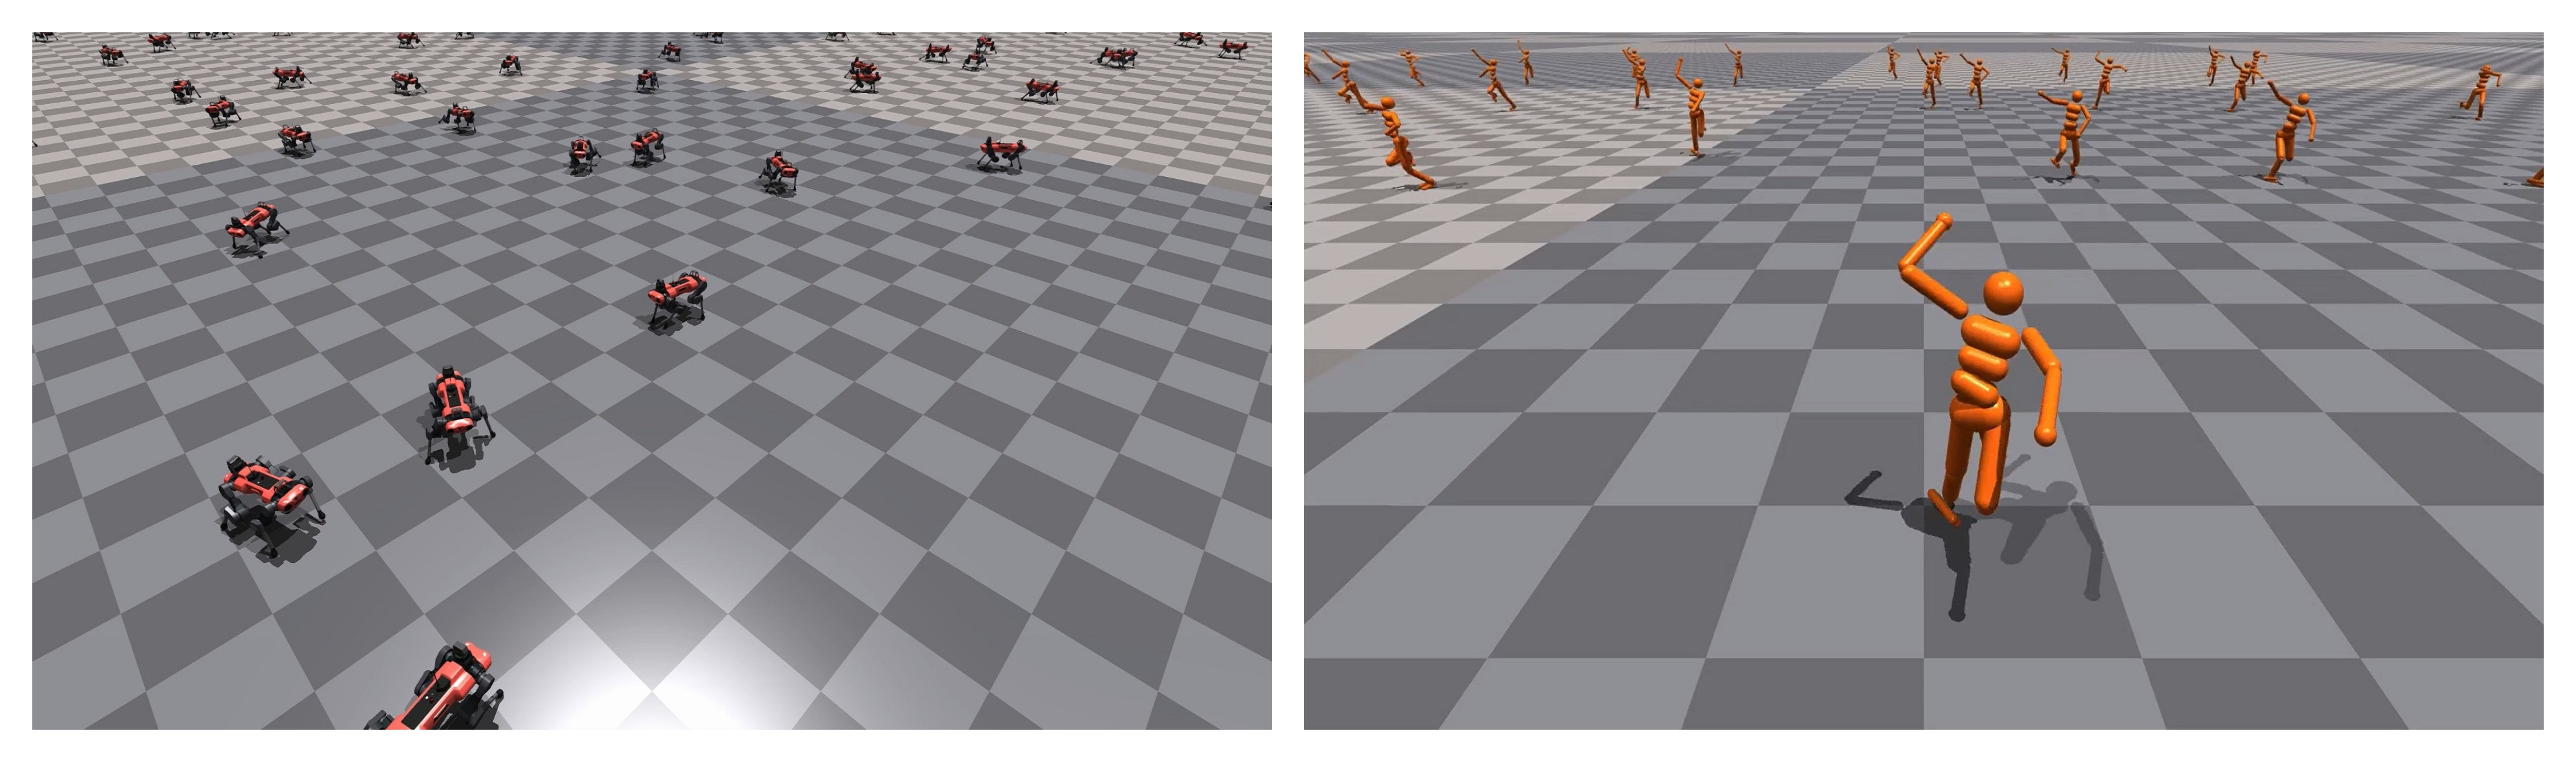
\includegraphics[width=\textwidth]{figures/chapter_intro/issac_gym.jpg}
% \caption{NVIDIA Isaac Gym}
% \label{fig.issac_gym}
% \end{figure}

% However, reinforcement learning models are vulnerable to adversarial attacks by adding perturbations to agents' observations \citep{chen2019adversarial}. Besides, recent research unveils that adversarial policy that acts abnormally in a shared environment can also induce extremely unlikely activations to occur.

% \begin{figure}[H]
% \centering
% 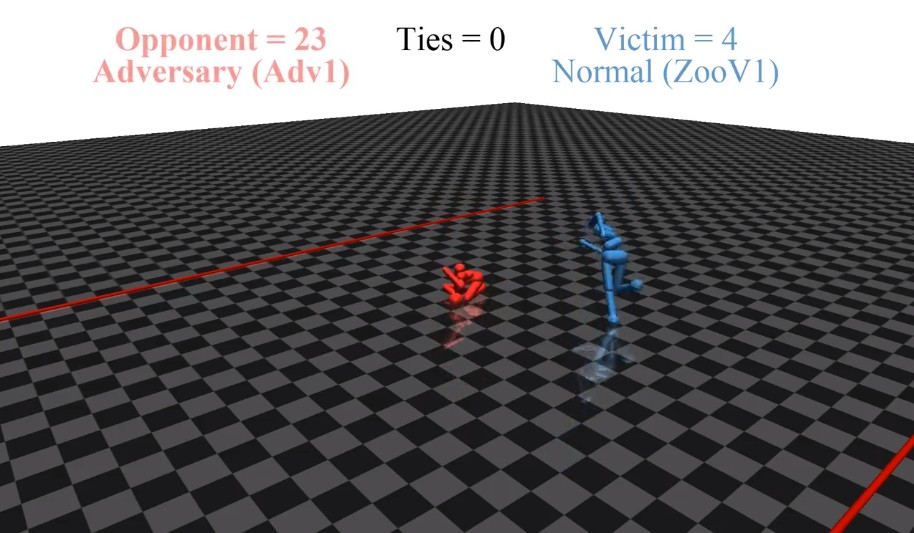
\includegraphics[scale=0.4]{figures/chapter_intro/adv_policy.jpg}
% \caption{Adversarial Policies: Attacking Deep Reinforcement Learning}
% \label{fig.adv_policy}
% \end{figure}

% For instance, the red agent tries to prevent the blue agent from crossing the line. Unexpectedly, the red agent wins the game by falling to the ground, which looks like a random policy. But this abnormal action of the red agent effectively causes the blue agent to fall as well \citep{gleave2021adversarial}. 

% In chapter \ref{chpt:driving}, we provide more experiments of adversarial attacks against end-to-end models in autonomous driving systems.

Unfortunately, both modular systems and end-to-end driving models are vulnerable to adversarial attacks. The trustworthiness of deep learning models for medical diagnoses is also challenged.

% \clearpage

\section{Adversarial Attacks}
\label{sec:adv_attack}

The existence of adversarial examples was first identified by Biggio et al. \citep{biggio2013evasion}, and Szegedy et al. \citep{szegedy2013intriguing}, in which they fooled a classification model by adding a small perturbation to the input image. Existing adversarial attacks can be categorized into white-box, gray-box, and black-box attacks. 

In white-box attacks, the adversaries have full knowledge of the target model, including the model architecture and parameters. In gray-box attacks, the adversaries only have limited access to the training set, model structure, model parameters, and model outputs. In black-box attacks, the adversaries can only gather information about the target model through querying \citep{REN2020346}. This thesis focuses on white-box and black-box attacks because the boundary between gray-box and black-box attacks is unclear. For instance, gray-box attacks with no access to predicted probabilities are also known as label-only black-box attacks.

% Depending on the goal of the attack, adversarial attacks can be further categorized into three types, evasion, poisoning, and extraction attacks \citep{art2018}. Evasion attacks cause models to make incorrect predictions by adding perturbations to the input during inference. The poisoning attack injects malicious data into the training set. Lastly, the extraction attack steals or replicates models that are available to query. For autonomous systems, rather than trying to steal models or poison others' training data, we intend to design a system that is resistant to malicious perturbations in the input. Thus our research object coincides with evasion attacks.

\subsection{White-Box Attacks}
\label{sec:whitebox_attack}

White-box attacks rely on gradients to fool deep-learning models. Different attack methods use different loss functions to compute the gradient, thus achieving different attack objectives. The strategy of updating and applying the perturbation also varies. Next, we use image classification models as target models to illustrate the general idea of white-box adversarial attacks (see Fig. \ref{fig.adv_perturb}).

\begin{figure}[H]
\centering
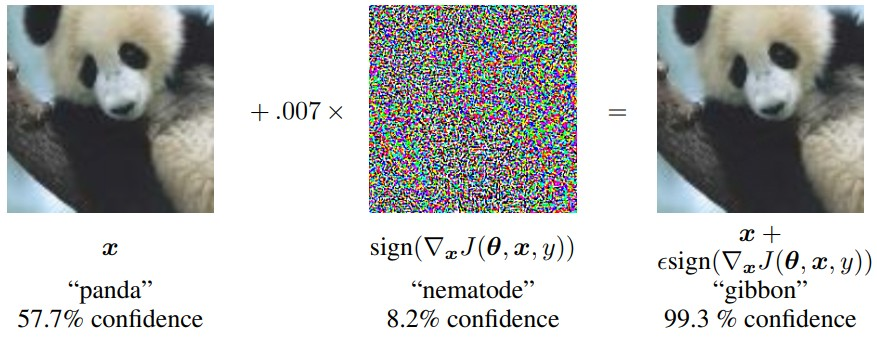
\includegraphics[width=0.95\textwidth]{figures/chapter_intro/fgsm.jpg}
\caption{The \acrfull{fgsm}\citep{goodfellow2015explaining} is the first gradient-based white-box attack.}
\label{fig.adv_perturb}
\end{figure}

\subsubsection{Problem Formulation}

Taking image classification models as an example, the deep learning model is denoted as $f(\cdot)$ with input $x$ and prediction $f(x, \theta)$, where $\theta$ is the model weights. The corresponding optimization loss is denoted by $\mathcal{L}(f(x, \theta), y^*)$, where $y^*$ is the ground truth. An adversarial input $x'$ is close to the original input $x$ under a specific distance metric while $f(x', \theta) \neq f(x, \theta)$. Formally, an adversarial example is defined as follows:

\begin{equation}
x^{'}: ||x - x^{'}|| < \eta, f(x', \theta) \neq f(x, \theta)
\end{equation}

where $ \eta $ is a predefined distance constraint on the maximum allowed perturbation. The most commonly used distance metric is the $L_p$ distance metric. The distance between $x$ and $x'$ is denoted as $||x-x'||_{p}$, where $||\cdot||_p$ is defined as follows:

\begin{equation}
 ||\textbf{v}||_p = (|v_1|^p + |v_2|^p + \dots + |v_d|^p)^{1/p}
\end{equation}
where $p$ is a real number and $d$ is the dimension of the vector $\textbf{v}$. For instance, the $L_0$ distance corresponds to the number of pixels being modified in the perturbation. The $L_2$ distance measures the standard Euclidean distance between $x$ and $x'$, and the $L_\infty$ distance measures the maximum element-wise difference between $x$ and $x'$.

With full access to model structure and parameters, white-box attacks \textbf{maximize} the loss function  $\mathcal{L}(f(x, \theta), y^*)$ by adding noises to \textbf{ model inputs} $x$, while deep learning models are trained by \textbf{minimizing} the loss function  $\mathcal{L}(f(x, \theta), y^*)$ via updating \textbf{model weights} $\theta$.

\subsubsection{Adversarial Perturbation}

The first gradient based white-box attack is the \acrfull{fgsm} \citep{goodfellow2015explaining} that generates the adversarial input using:

\begin{equation}
x' = x + \eta \cdot \text{sign}(\ \bigtriangledown_x \mathcal{L}(f(x, \theta), y^*)\ )    
\end{equation} 

where $\text{sign}(\cdot$) calculates the element-wise sign of a given matrix and $\bigtriangledown_x \mathcal{L}(f(x, \theta), y^*)$ is the gradient of the input $x$ with respect to the loss $\mathcal{L}(f(x, \theta), y^*)$.

The \acrshort{fgsm} generates the adversarial example in one step, while the \acrfull{pgd} \citep{madry2017towards} transforms the \acrshort{fgsm} attack into a multi-step attack that updates the perturbation at each iteration while keeping the overall perturbation $x^{'}$ in a $L_p$ ball using the projection function $\texttt{proj}_{p}(\cdot)$:

\begin{equation}
x'_{t+1} = \text{proj}_{p}(x'_t + \eta \cdot \text{sign}(\ \bigtriangledown_x \mathcal{L}(f(x, \theta), y^*)\ ))
\end{equation}

% \clearpage

\subsubsection{\acrfull{uap}}

The multi-step \acrshort{pgd} attack is further improved by the Deep Fool attack \citep{moosavidezfooli2016deepfool} that adds the norm of the gradient difference while iterating over each class $k$ at each step $t$:

\begin{equation}
x'_{t+1} = x'_t + \frac{|f_k(x^{'}_{t}, \theta) - f_{k^{*}}(x^{'}_{t}, \theta)|}{||\omega'_{\hat{k}}||^2_2} \text{sign}(\omega'_{\hat{k}})
\end{equation}

where the $k^*$ is the ground truth class label and $x_0$ is the original input image without adversarial perturbations. $\omega'_k$ is the gradient difference between the gradient calculated using the original image and the adversarial image:  $\omega'_k = \bigtriangledown_x \mathcal{L}(f(x', \theta), y^*) - \bigtriangledown_x \mathcal{L}(f(x_0, \theta), y^*)$.

\textbf{From image-specific attack to image-agnostic attack:} So far, we have only introduced image-specific attacks that generate adversarial perturbation for each input image. As image-specific attacks become more and more effective while keeping human-unperceivable, another research question arises: can we produce an image-agnostic perturbation that can attack all images in a dataset?

Based on the Deep Fool attack, Moosavi-dezfooli et al. generate \acrshort{uap}s, represented with $\textbf{v}$, by further projecting the overall perturbation to $L_p$ ball of radius $\epsilon$ and centered at 0 after iterating over each class $k$ \citep{moosavidezfooli2017universal}:

\begin{equation}
\text{proj}_p(\textbf{v}, \epsilon)= \arg\ \underset{\textbf{v}_{t+1}}{\min}||\textbf{v}_{t+1} - \textbf{v}_{t}||_2 \quad \text{subject to}\ ||\textbf{v}_{t+1}||_p\leq\epsilon
\end{equation}

\begin{figure}[H]
\centering
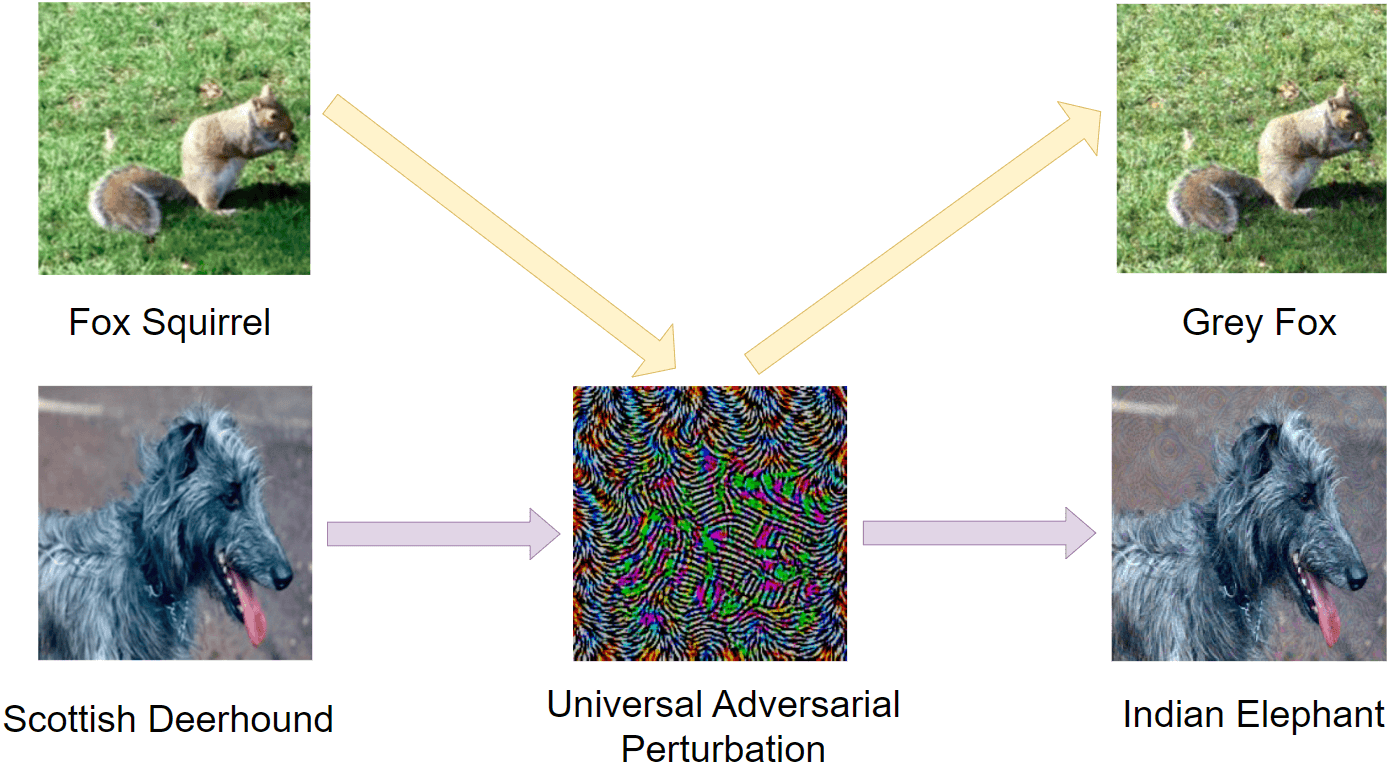
\includegraphics[width=0.9\textwidth]{figures/chapter_intro/uap.png}
\caption{The \acrfull{uap} attacks different images using the same perturbation.}
\label{fig.uap}
\end{figure}

% \clearpage

\subsubsection{Adversarial Patch (Digital)}

As illustrated in previous sections, adding a small and intentional drift to the input distribution, also known as adversarial perturbations, can substantially decrease the deep neural network's performance. However, the effectiveness of the adversarial perturbation is limited by the maximum allowed perturbation. What if the adversaries prioritize the attack success rate over imperceptibility, which means we can remove the constraint of imperceptibility?

Other than applying a small adversarial perturbation to the entire image, we can also add a human-noticeable patch to a small region of the input image to opt for a more effective (see Fig. \ref{fig:digital_patch}). Besides, the effectiveness of adversarial patches should be position invariant. Digital patches can fool the model without overlapping with target objects \citep{saha2019adversarial}.


\begin{figure}[H]
\centering
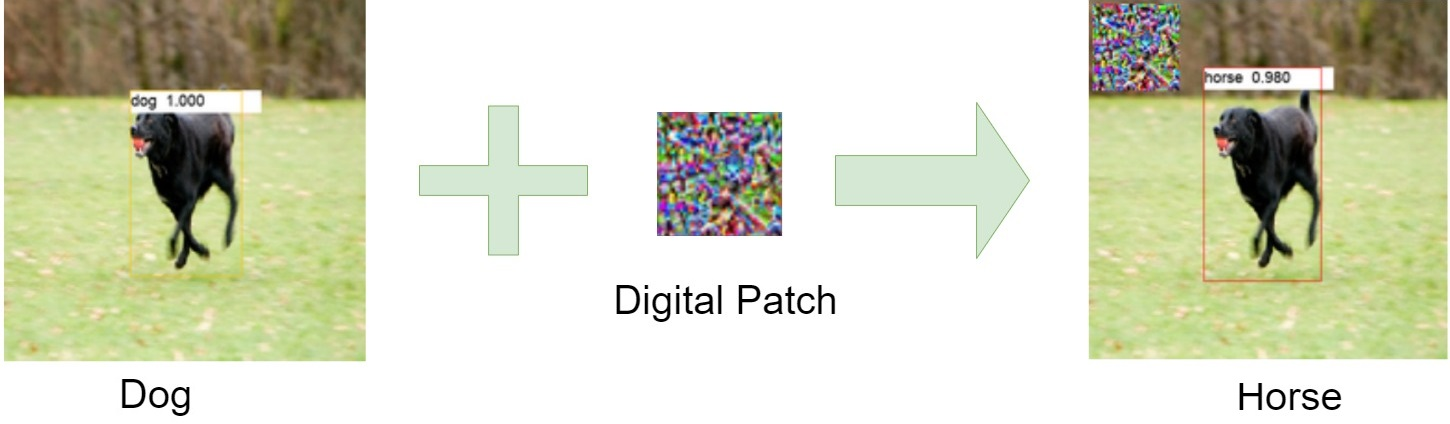
\includegraphics[width=0.95\textwidth]{figures/chapter_intro/digital_patch.jpg}
\caption{The digital patch attacks the image by modifying pixel values.}
\label{fig.digital_patch}
\end{figure}


% A variant of the Expectation over Transformation (EOT) framework \citep{athalye2018synthesizing} is used to obtain the trained patch. In particular, the patch is trained to optimize the objective function:

% $$\hat{p} = \arg \underset{p}{\max}\mathbf{E}_{x \sim X, t \sim T,l \sim L}[logPr(\hat{y}|A(p,x,l,t))]$$

% where $X$ is a training set of images, $T$ is a distribution over transformations of the patch, and $L$ is a distribution over locations in the image \citep{brown2018adversarial}.

% \clearpage

\subsubsection{Adversarial Patch (Physical)}

Digital patches apply adversarial perturbations by directly modifying image pixel values. In 2017, Brown et al. brought adversarial examples to the physical world by printing human-noticeable patches on stickers \citep{brown2017adversarial}, posing threats against real-world applications (see Fig. \ref{fig.physical_patch}). The physical patch is trained using 10,000 images from the training set, applying a random translation, scaling, and rotation on the patch in each image.

Later, research interests gradually shifted from digital attacks to physical attacks. In 2019, the digital DPatch \citep{liu2018dpatch} was extended to the physical world \citep{lee2019physical} by adding expectation over transformations.

\begin{equation}
\hat{p} = \arg \underset{p}{\max}\mathbf{E}_{x \sim X, t \sim T}\ \mathcal{L}[f(A(x', p, t), \theta), y^*]
\end{equation}

where $A(\cdot)$ is a “patch application function” that transforms the patch
$p$ with the transformation $t$ sampled from a series of transformations $T$.

\begin{figure}[H]
\centering
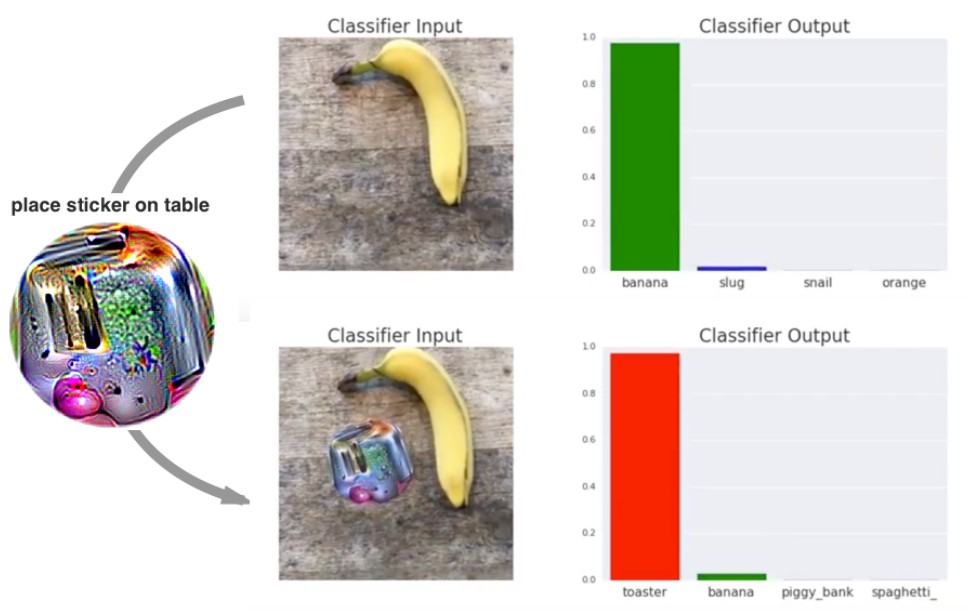
\includegraphics[width=\textwidth]{figures/chapter_intro/adv_patch.png}
\caption{Physical Patch: the adversarial patch is printed and placed on the table \citep{brown2017adversarial}.}
\label{fig.physical_patch}
\end{figure}

The physical patch can be further improved by adding the \acrfull{nps} as extra constraints to the optimization loss function:

\begin{equation}
\hat{p} = \arg \underset{p}{\max}\mathbf{E}_{x \sim X, t \sim T}\ \mathcal{L}[f(A(x', p, t), \theta), y^*] + SNPS(p, \beta)
\end{equation}

where $\beta$ is the sampling rate and the \acrfull{snps} is used to measure the image printability, or in other words, the error between a printed pixel and its digital counterparts \citep{wang2021daedalus}. However, some research generates asterisk and grid-shaped patches \citep{wu2020dpattack} or small patches \citep{huang2021rpattack} to reduce the number of perturbed pixels, making it infeasible to be printed out on physical objects.

The reason that physical patches are visually perceptible by human eyes is that they must be able to be captured by sensors (e.g. cameras). As a result, physical attacks require a substantial intensity of perturbations. In a survey on physical attacks, Wei et al. categorized adversarial patches into meaningful patches and meaningless patches that do not correspond to real-world objects \citep{wei2023visually}. For example, Chindaudom et al. produce meaningful patches by combining patches with QR Codes \citep{chindaudom2020adversarialqr, chindaudom2022surreptitious}. 

\begin{figure}[H]
\centering
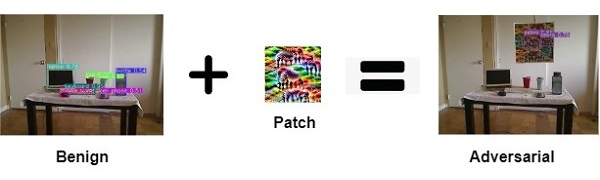
\includegraphics[width=\textwidth]{figures/chapter_intro/physical_patch.png}
\caption{The physical patch can either be attached on the target object or does not overlap with target objects.}
\label{fig.physical_patch_overlap}
\end{figure}

Physical patches pose great threats against autonomous driving vehicles because they are invariant to input images and thus can inherently achieve real-time attacks \citep{threet2021physical}. For instance, prior research generates stop signs that cannot be recognized by object detection models \citep{song2018physical} \citep{chen2019shapeshifter}, and adversarial posters to vanish pedestrian \citep{thys2019fooling, wang2021towards}. Besides, physical patches do not necessarily need to overlap with target objects (see Fig. \ref{fig.physical_patch_overlap}).

Though most patches are static, Hoory et al. generate and display dynamic patches on a monitor attached to a vehicle \citep{hoory2020dynamic}. However, physical patches can only attack object detection models when the camera is close enough \citep{wang2021daedalus, lu2021scale}.

On the other hand, though most physical attacks are visually perceptible by human eyes, some optical attacks can only be captured by sensors (e.g., rolling shutter attacks) but not by human eyes. Li et al. summarized optical adversarial attacks, including attacks that use high-frequency light, laser, and projector in \citep{li2022survey}.

% Our research will focus on adversarial patches that are noticeable by human eyes. In \cite{sharma2022adversarial}, Sharma et al. surveyed adversarial patch attacks in vision-based tasks that involve three mainstream models: classification, detection, and re-identification \cite{wei2022physical}, and we will focus on adversarial attacks against object detection models.

% \clearpage

\subsection{Black-Box Attacks}
\label{sec:blackbox_attack}

White-box attacks that rely on gradients can generate adversarial examples efficiently. However, gradients are not available for real-world deep learning applications because gradients are essential only for training but not for inference. Real-world applications that only perform the inference do not compute gradients. 

Without access to gradients, white-box attacks become infeasible in the real world. As a result, black-box attacks become promising for attacks against deep learning cloud services.


\subsubsection{Problem Formulation}

Taking black-box attacks against image classification models as an example, the adversary has no access to the model structure and model weights and can only generate adversarial perturbations via sending queries to the model (see Fig. \ref{fig.decision}).
 
Given an input image $x$ and the true label $x$, the objective of the adversary is to fool a black-box image classifier $f(x)$ by adding a small perturbation $\delta$ to the original image, and generate an adversarial image $x^{'} = x + \delta$, such that $f(x^{'}) \neq f(x)$. Typically, the perturbation $\delta$ is bounded in the $l_2$ or $l_{\infty}$ norm by some user-defined constant.

Decision-based black-box attacks only require access to the predicted class (hard label), while score-based attacks also require the probability of each predicted class (soft label).  Next, we introduce the two most popular strategies of black-box attacks: gradient estimation and local search.

\begin{figure}[H]
\centering
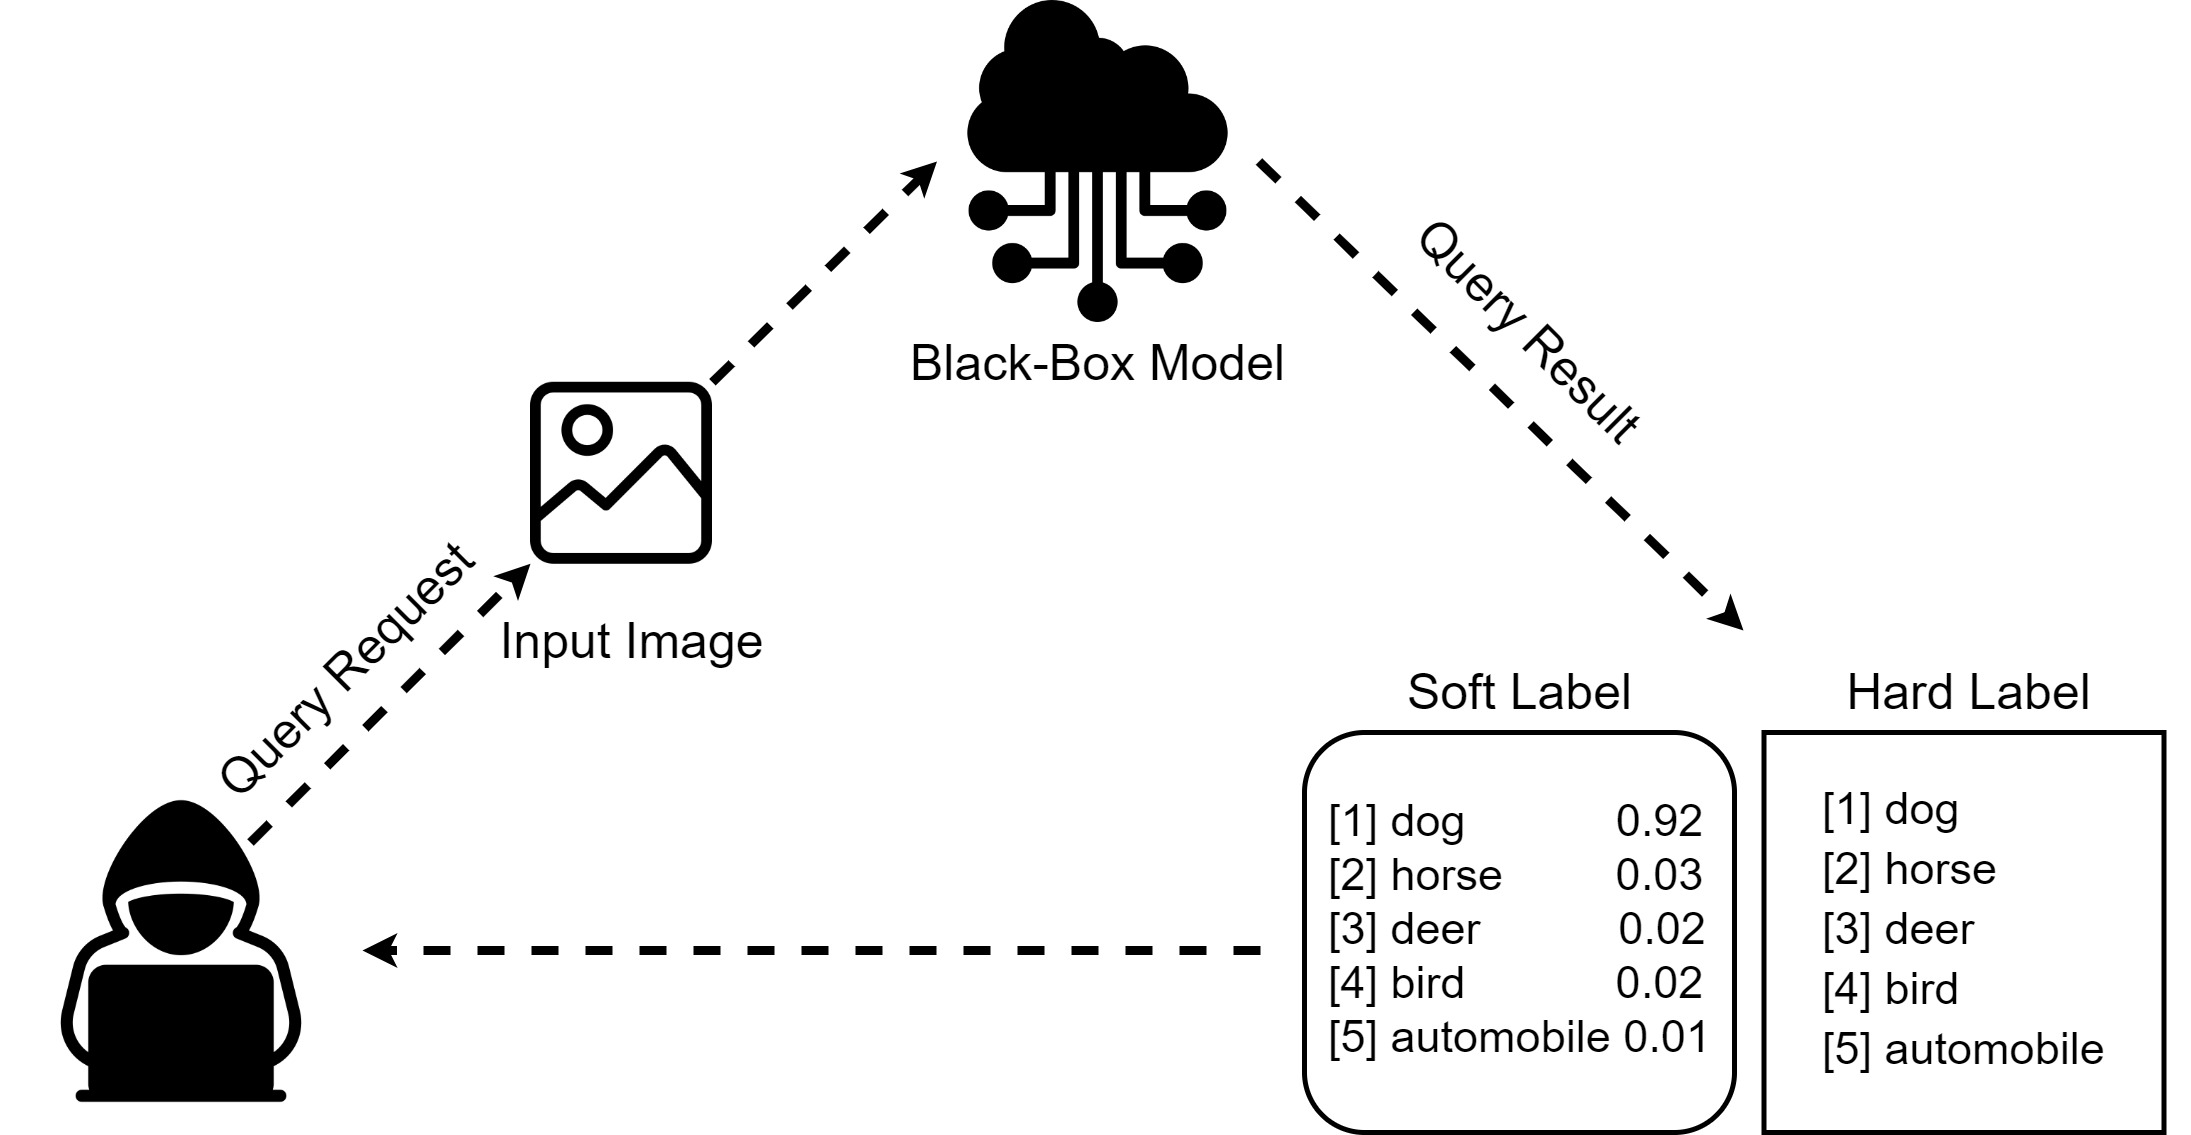
\includegraphics[width=\textwidth]{figures/chapter_intro/black-box.jpg}
\caption{The Black-Box Adversarial Attack.}
\label{fig.decision}
\end{figure}

\clearpage

\subsubsection{Gradient Estimation}

Intuitively, if we can estimate gradients, we can exploit existing white-box attacks to generate adversarial examples. For instance, the \acrfull{zoo} Attack amends the C\&W white-box attacks to the black-box setting by modifying the loss function and computing an approximate gradient using a finite difference method \citep{Chen_2017}. The original C\&W attack generates adversarial examples $x'$ by solving the optimization problem:

\begin{equation}
    \text{minimize}\ ||x'-x||^2_2 + c \cdot F(x', t)
\end{equation}

where $F(x', t)$ is the regularization function and $c>0$ is a regularization parameter. The target class is represented with $t$.

To solve the above optimization problem, we need access to gradients of the regularization function with respect to the input $\bigtriangledown_{x^{'}} F(x^{'}, t)$, which is not available under black-box settings. Thus, the \acrshort{zoo} attack estimates the gradient using a finite difference method rather than backpropagation:

\begin{equation}
    \frac{\partial F(x)}{\partial x} \approx \frac{F(x+he_i) - F(x-he_i)}{2h}
\end{equation}

% \begin{equation}
%     \frac{\partial^2 F(x)}{\partial x^2} \approx \frac{F(x+he_i) - 2F(x) + F(x-he_i)}{h^2}
% \end{equation}

where $h$ is a small step size (e.g. $h = 0.0001$), and $e_i$ is a standard basis vector with only the i-th component being 1.

Query efficiency is a crucial evaluation metric for black-box attacks, and the following research tries to improve the sample efficiency of gradient estimation using gradient priors and natural gradient estimation.

% \begin{equation}
% f(x,t) = \max \{ {\underset{i \neq t}{\max}\ log[F(x)]_i - log[F(x)]_t, -\kappa } \}
% \end{equation}

% The ZOO Attack relies on the output of confidence scores to estimate the gradient, while decision-based attacks can generate adversarial inputs using even less information.

\subsubsection{Local Search}

On the other hand, local search is another popular black-box attack method. The FGSM attack either adds or deducts a small value to each pixel, indicating that adversarial perturbations are combinations of orthogonal vectors. As a result, local search methods use existing local search methods, such as heuristic search, to search for combinations of orthogonal vectors to decide what pixels to attack.

Intuitively, we can add or deduct a small value to one pixel at a time and choose the operation that decreases the probability of the correct label. The attack is known as the \acrfull{simba} \cite{guo2019simple}, a baseline method. However, even for a 32x32 input image, the \acrshort{simba} method takes over 2000 queries, which is inefficient. To reduce the search space, later research finds combinations of vertical and horizontal lines and square patches rather than individual pixels.

\clearpage

Besides gradient estimation and local search, another approach to produce adversarial examples is to use a surrogate model. Surrogate-based black-box attacks generate adversarial perturbations by transferring from a surrogate model, but their attack success rates are lower than gradient-estimation and search-based methods.

Though existing black-box attacks achieve remarkable attack success rates, we notice some common mistakes in prior research that obtain unfair advantages by applying the perturbation before image encoding and pre-processing. We introduce these common mistakes in Chapter \ref{chpt:classification}.

\section{Research Questions}
\label{sec:research_question}

Despite rapid progress in generating adversarial examples, there are many important questions arising for practical adversarial attacks.

\vspace{0.5cm}

\textbf{Can we achieve real-time online adversarial attacks?}

Much of the current research in adversarial attacks focuses on offline attacks that utilize both input images $x$ and corresponding ground truths $y^*$ to maximize the adversarial loss $\mathcal{L}(f(x, \theta), y^*)$. However, the human-labeled ground truth $y^*$ is unavailable for real-time online attacks. For example, to attack an object detection model deployed on an autonomous driving vehicle, it is impossible to have humans mark the bounding boxes in real time. Can we generate adversarial perturbations without access to the ground truth?

\vspace{0.5cm}

\textbf{Can we inject the perturbations without access to the operating system?}

Access to the operating system is essential in order to inject adversarial perturbations into input images. However, the operating system (Unix/Linux) where the deep learning model is deployed is highly secure as research in cyber security advances. Although the operating system is highly secure, the sensors that collect the data are exposed directly to the environment to collect the data. Can we exploit the sensor to bypass the operating system?

\vspace{0.5cm}

\textbf{Can traditional methods mediate the impact of adversarial attacks?}

Although deep neural networks are vulnerable to adversarial attacks, traditional algorithms such as the Kalman Filter and the Hungarian algorithm are not. In real-world robotic applications, deep learning models are deployed in combination with traditional algorithms that do not use deep neural networks. Are adversarial attacks still effective under these settings?

\vspace{0.5cm}

\textbf{Have black-box attacks become a practical threat against cloud APIs?}

IoT devices that do not have enough memory and computational resources rely on cloud APIs to achieve computer vision tasks, such as image classification. Have existing black-box attacks become a real threat against cloud APIs?

\vspace{0.5cm}

\textbf{How can we embrace deep learning models safely?}

Deep learning models that achieve high accuracy provide fewer interpretations due to the trade-off between accuracy and interpretability. How can we interpret and safely embrace black-box models, especially for medical applications?

% It is risky to put one's life in the hands of models that medical researchers do not fully understand. 

% \clearpage

\section{Thesis Overview}

To answer the research questions listed in Section \ref{sec:research_question}, the remaining of the thesis is organized as follows:

% This thesis presents adversarial attacks against mobile robot perception models, such as image classification, object detection, and object tracking. 

\begin{itemize}[label={}]
    \item \textbf{Chapter \ref{chpt:driving}} introduces the real-time online white-box attack against the NVIDIA end-to-end driving model. The attack does not require access to the ground truth (\textbf{Published in IEEE Intelligent Vehicle Symposium}).
    \item \textbf{Chapter \ref{chpt:detection}} further presents real-time online white-box attacks against object detection models (\textbf{Published in IEEE Intelligent Vehicle Symposium}). Besides, we propose a Human-in-the-Middle hardware attack that injects the perturbation into the communication channel between the camera and the detection system (\textbf{IEEE Transactions on AI, minor revision}).
    \item \textbf{Chapter \ref{chpt:tracking}} attacks the object tracking system.

    To be done.

    To be done.

    \item \textbf{Chapter \ref{chpt:classification}} unveils several common mistakes in prior research and proposes distributed black-box attacks to accelerate attacks against image classification cloud services (\textbf{Under Review}).
    \item \textbf{Chapter \ref{chpt:defence}} studies the interpretability of machine learning models for medical applications and combines deep neural networks with human knowledge to understand how black-box models make diagnosis (\textbf{Published in IEEE Transactions on AI}).
    \item \textbf{Chapter \ref{chpt:conclusion}} concludes the thesis and envisions future research directions to understand and safely embrace deep learning models. 
\end{itemize}

% Since end-to-end deep learning models are computationally expensive, pruning and quantization are commonly used techniques to make large models feasible for embedded systems, but theses techniques could render deep learning models more vulnerable.

